%CaseQuad%
Air Traffic Control (ATC) offers many opportunities for automation to allow safer and more efficient landing patterns. 
The constraints of ATC are complex and contain many safety rules \cite{Max_ICRAT16}.
%\cite{JohnsonICCPS12}, \cite{Max_ICRAT16}.
In this example we formalize a subset of such rules, similar to those in example \ref{ex:ATC_example}, for an autonomous ATC for quad-rotors in MTL.
We demonstrate how the smoothed robustness is used to generate control strategies for safely and robustly manoeuvring two quad-rotors in an enclosed airspace with an obstacle. 

\textbf{The specification}.
The specification for the autonomous ATC with two quad-rotors is:
{\footnotesize
\begin{subequations}
\begin{align}
\formula &= \eventually_{[0,N-1]}(q_1 \in \text{Terminal}) \land \eventually_{[0,N-1]}(q_2 \in \text{Terminal}) \land   \nonumber \\
& \always_{[0,N-1]} (q_1 \in \text{Zone}_1 \implies z_1 \in [1,5]) \, \land \nonumber \\
& \always_{[0,N-1]} (q_2 \in \text{Zone}_1 \implies z_2 \in [1,5]) \, \land \nonumber \\
& \always_{[0,N-1]} (q_1 \in \text{Zone}_2 \implies z_1 \in [0,3]) \, \land \nonumber \\
& \always_{[0,N-1]} (q_2 \in \text{Zone}_2 \implies z_2 \in [0,3]) \, \land \nonumber \\
& \always_{[0,N-1]} (\neg (q_1 \in \text{Unsafe})) \land \always_{[0,N-1]} (\neg (q_2 \in \text{Unsafe})) \, \land  \nonumber \\
& \always_{[0,N-1]} (||q_1-q_2||_2^2 \geq d_{min}^2)
\end{align}
\end{subequations}
\vspace{-10pt}
}

Here $q_1$ and $q_2$ refer to the position of the two quad-rotors in $(x,y,z)$-space, and $z_1$ and $z_2$ refer to their altitude. 
The specification says that, within a horizon of $N$ steps,  both quad-rotors 
should: 
a) Eventually visit the terminal zone (e.g. to refuel or drop package), 
b) Follow altitude rules in two zones, $\text{Zone}_1$ and $\text{Zone}_2$ which have different altitude floors and ceilings,
c) Avoid the $\text{Unsafe}$ set, and d) always maintain a safe distance between each other ($d_{min}$). 

\textit{Note that turning the specification into constraints for the control problem is no longer simple.}
This is due to the $\eventually$ operator, which would require a MILP formulation to be accounted for. 
In addition, the minimum separation and altitude rules for the two zones cannot be turned into convex constraints for the optimization. As will be seen below, our approach allows us to keep the non-convexity in the cost function, and have convex (linear) constraints on the optimization problem.

\textbf{System dynamics.}
The airspace and associated sets for the specification $\formula$ are hyper-rectangles in $\mathbb{R}^3$ (visualized in Fig.~\ref{fig:quad_ssqp}), except the altitude floor and ceiling limit, which is in $\mathbb{R}^1$. In simulation, $d_{min}$ is set to $0.2$ m.
%These sets are visualized in Fig.~\ref{fig:quad_ssqp}. In simulation, $d_{min}$ is set to $0.2$ m.

%a hyper-rectangle in $\mathbb{R}^3$, $[-5,5] \times [-5,5] \times [0,5]$.
%The two quadrotors must start in $\text{Zone}_1 = [-5,0] \times [-5,5] \times [0,5]$, which has a %ceiling of $5$m and an enforced floor of $1$m. 
%They must eventually reach the terminal set, which is given by $\text{Terminal} = [3,4] \times %[3,4] \times [0,1]$.
%The terminal set resides in $\text{Zone}_2 = [0,5] \times [-5,5] \times [0,5]$, which has a ceiling of $3$m and a floor of $0$m.
%Finally, the $\text{Unsafe}$ set is a hyper-rectangle $[-1,1] \times [-1,1] \times [0,5]$ in the middle of the airspace. In simulation, $d_{min}$ is set to $0.2$ m.
%\todo[inline]{we might remove some of these dimensions to reduce space, since thee figure shows the sets...}

%This arrangement of the air-space, where the specifications for altitude ceiling and floors for either zone are in a $A \implies B$ format, is common in ATC (e.g. If holding in progress, go to holding zone and follow holding zone rules) and also allows us to combine the $\text{Airspace}$ with velocity-limits ($[-5,5]^3$) into the set $X$, which is a convex (Polyhedron) set constraint on the state of both quad-rotors, as will be explained below.
%\todo[inline]{unnecessary paragraph}

The quad-rotor dynamics are obtained via linearization around hover, and discretization at $5$-Hz. Similar models have been used for control of real quad-rotors with success (\cite{PantAMNDM15_Anytime}). For simulation, we set the mass of either quad-rotor to be $0.5$ kg. %and $g=9.8\,ms^{-2}$.
The corresponding linearized and discretized quad-rotor dynamics are given in \cite{PantAM17_SmoothOpTechRpt}.	The state for a quad-rotor $x \in \mathbb{R}^6$ consists of the velocities and positions in the $x,y,z$ co-ordinates respectively. 
The inputs to the system are the desired roll angle $\theta$, pitch angle $\phi$ and thrust $\text{T}$. 

%as:

%{\tiny
%\vspace{-10pt}
%\begin{equation}
%\label{eq:quad_dyn}
%\begin{bmatrix} \dot{x}_{k+1} \\ \dot{y}_{k+1} \\ \dot{z}_{k+1} \\ x_{k+1} \\ y_{k+1} \\ z_{k+1} \end{bmatrix}= \begin{bmatrix} 1&0&0&0&0&0 \\0&1&0&0&0&0 \\0&0&1&0&0&0 \\0.2&0&0&1&0&0 \\0&0.2&0&0&1&0 \\0&0&0.2&0&0&1\end{bmatrix} \begin{bmatrix} \dot{x}_{k} \\ \dot{y}_{k} \\ \dot{z}_{k} \\ x_{k} \\ y_{k} \\ z_{k} \end{bmatrix} + \begin{bmatrix} 1.96&0&0 \\ 0&-1.96&0 \\0&0&0.4 \\0.196&0&0 \\0&-0.196&0\\0&0&0.04 \end{bmatrix} \begin{bmatrix} \theta_k \\ \phi_k \\ \text{T}_k \end{bmatrix}
%\end{equation}
%\vspace{-10pt}
%}


%In a real system, this thrust is in addition to the hover thrust, $mg$, and a high-frequency low-level controller (not simulated) is responsible for generating rotor speeds to match the desired roll, pitch and thrust (with yaw set to be stabilized at $0$). 


%We solve the following control problem.
%\begin{subequations}
%\vspace{-10pt}
%\label{eq:atc_ctrl}
%\begin{align}
%\text{max } & \srob_{\formula}(\sstraj) \\ %- \gamma \sum_{k=0}^{N-1} l(x_{k+1},u_{k}) \\
%\text{s.t. } & x_{k+1} = f(x_k,u_k), \, \forall k=0,\dotsc,N-1 \\
% & x_k \in X, \, \forall k=0,\dotsc,N \\
% & u_k \in U, \, \forall k=0,\dotsc,N-1 
% & \delta \srob_{\formula}(\sstraj) \geq 0
%\end{align}
%\end{subequations}
\textbf{The control problem.} For the autonomous ATC problem for two quad-rotors, we solve \eqref{eq:general_ctrl}  with $\srob$ in the objective instead of $\rob$.
Note, we set $\gamma=0$ here, following logically from existing ATC rules (see sec.\ref{sec:intro}), which do not have an air-craft specific cost for fuel, or distance traveled. Because of this, we can also set $\delta=0$ and simply maximize (smooth) robustness (subject to system dynamics and constraints) to get trajectories that satisfy $\formula$.
% With some abuse of notation, for the control formulation, $x$ represents the concatenated state of the two quadrotors, and $u$ the concatenated inputs to the system. 
For the control problem ($P_{\srob}$), $X$ and $U$ represent the bounds on the states ($\text{Airspace}$ and velocity limits) and inputs respectively, for both quad-rotors. $f$ represents the linearized dynamics applied to two quad-rotors, and $N=21$. The initial state for the first quad-rotor is $[0,0,0,2,2,2]'$ and for the second, $[0 ,0 ,0,2, -2 , 2]'$.
%The control problem is to maximize the smooth robustness of the specification $\srob_{\formula}$, subject to the dynamics of two identical quad-rotors, and input limits of $0.5236$ radians (or $30$ degrees) on both roll and pitch, and $\text{T}\in[-1.5,1.5]$, giving us the set $U$. The set $X$ for state limits on either quadrotor is, as defined earlier, the Cartesian product of velocity limits $[-5,5]^3$ and the $\text{Airspace}$ set, i.e. $[-5,5]^3$. Also with respect to the general control problem, \eqref{eq:general_ctrl}, we set $\gamma=0$ and $\delta=0$. This keeps the smooth robustness only in the cost (to be maximized) and allows a fair comparison of the optimization of robustness with other methods. In general, our formulation has linear constraints (dynamics and $X$, $U$) for both quad-rotors, allowing us to easily apply off the shelf optimization solvers.
%\todo[inline]{repetitive. get to it. remove this paragraph and replace it with the control problem mathematically, as done for toy example.}
 %, Simulated Annealing and gradient descent, via SQP, on the robustness function.

%For simulation purposes, 
%\todo[inline]{what other purposes are there?}
%we obtain 3 initial trajectories (via solving different linear programs) from the given initial state to the terminal (landing) set. These three trajectories, each of which has negative robustness (i.e. does not satisfy the given specification), serve as three different initial solutions to A) Our approach B) Gradient-descent via SQP, using the actual robustness function as the cost, C) Simulated Annealing with the actual robustness function as the cost. This multi-start approach can be used in practice when there is a fast initial trajectory generator available.
%\todo[inline]{re-word in a much more direct style, as follows:}

\textbf{Results.}
For each approach (except BluSTL), we ran three optimizations, starting from three different trajectories to initialize the optimization. This can be thought of as a multi-start optimization, and these \textit{initial trajectories} can be obtained in practice by a fast trajectory generator. All three initial trajectories have negative robustness, i.e. they violate $\formula$.
In this case study, we only aim to maximize robustness, i.e. operate in the \textit{robust} mode. BluSTL, in either \textit{boolean} or \textit{robust} mode could not find a solution for this problem (ran over 100 hours without terminating) and so is excluded from the rest of this comparison. This suggests that having a complex specification like the one in this problem, non-trivial dynamics/horizon length results in a MILP that is intractable to solve. We believe that this example highlights a fundamental limitation of MILP based approaches.



%\begin{figure}[t]
%\centering
%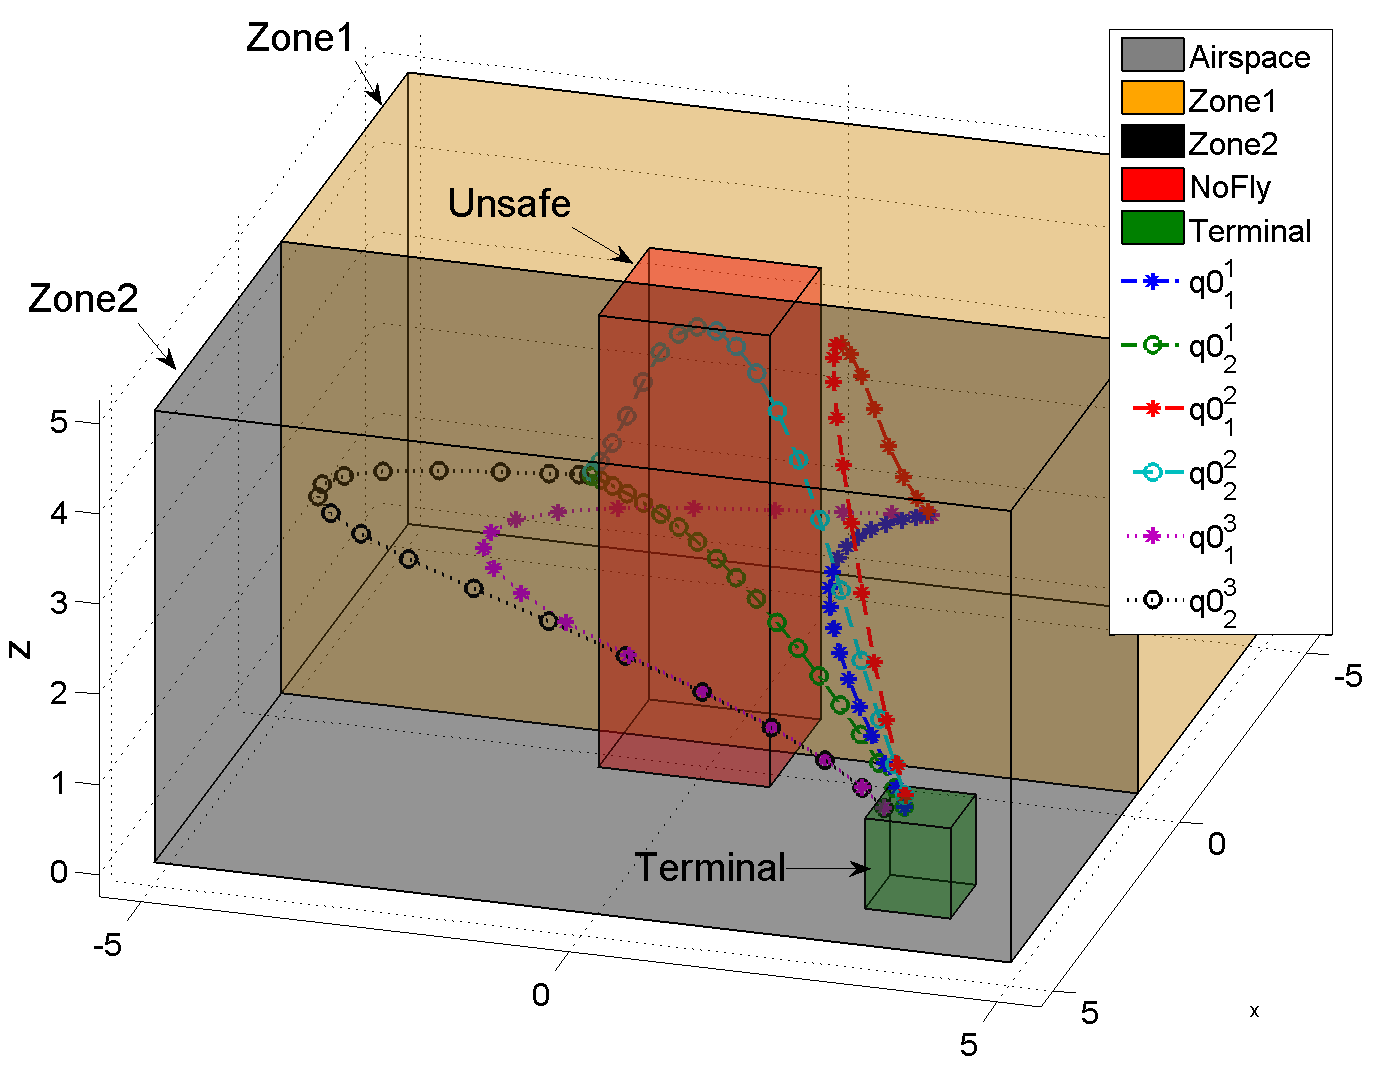
\includegraphics[width=0.49\textwidth]{figures/QuadInitTrajs_scissored}
%\vspace{-10pt}
%\caption{{\small The airspace with the corresponding sets, and initial trajectories for the two quad-rotors. Note, all 3 initial trajectories violate the specification, and the $\text{Airspace}$ is the union of $\text{Zone}_1$ and $\text{Zone}_2$. Here, $q0_{i}^j$ refers to the positions of the $i^{th}$ initial trajectory for the $j^{th}$ quadrotor.}}
%\label{fig:quad_init}
%\vspace{-10pt}
%\end{figure}
%Fig.\ref{fig:quad_init} shows the initial trajectories for both the quadrotors in the given air-space, neither of which satisfy the specification $\formula$. 
%Fig.\ref{fig:quad_ssqp} shows the three trajectories obtained after applying SOP,
%with the three initial trajectories as initial guesses for the optimizations. 
%\todo[inline]{use the names of the methods, here, SOP} 
%\todo[inline]{it's either a trajectory or a point. the reader can't peer into your head and see that you're thinking about them in the ssame way. Stick to one nomenclature, "initial trajectory". moreover, we've already explained above what an initial rajectory is, so we don't have to keep explaining that it initializes the optim.}
%for the optimization, respectively. 
Fig.\ref{fig:quad_ssqp} shows the three trajectories obtained after applying SOP, all of which satisfy the specification $\formula$. 
To avoid visual clutter, we do not show the trajectories obtained from the other methods on the figure.
Instead, we summarize the results in Table \ref{tbl:opt_performance} which shows the true robustness of the three initial trajectories, and the true robustness for the trajectories obtained via the three methods, SOP, SA, and R-SQP. %In order to keep the study easy to interpret, we use two quad-rotors, but it is straight forward to scale the specification and the optimization to account for more. 
Unlike previous examples, we did not explicitly compute the gradient of the robustness for $\formula$. Because of this run-times are much slower as MATLAB has to numerically compute the gradient using finite-differences, resulting in overheads that were not incurred in the other examples. Despite this, SOP takes the order of 30 minutes for the optimization, while SA and R-SQP take over 4 hours to do so. Including explicit gradients should result in a significant speed up as was observed for the other examples. 


%Our method, SQP with Smooth Robustness (SOP)
%\todo[inline]{define once, use forever: SOP}, 
%results in trajectories with the highest robustness.
%SA, with an upper limit of 30,000 function evaluations, results in only one trajectory that satisfies $\formula$. 
%SQP on robustness 
%\todo[inline]{chicken on rice. R-SQP}
%results in trajectories that satisfy $\formula$ from all 3 initial trajectories. 
%R-SQP consistently returns lower values of robustness than SOP, but also from three very different initial trajectories, 
%\todo[inline]{"very" initial?}
%\todo[inline]{re-organize: SOP and R-SQP satisfies the spec every time, SA only once.
%	\\ SOP gives highest robustness values, higher than R-SQP.
%	\\ observations below about getting stuck at local minima due to non-diff. }
%results in trajectories with the same robustness value $0.1798$. 

\textbf{Analysis.} It is seen that SOP and R-SQP satisfy $\formula$ for all instances, while SA satisfies it only once.
Note that in all three cases, R-SQP results in trajectories with the same robustness value, which is less than the robustness value achieved in SOP.
We conjecture that this is because R-SQP is getting stuck at local minima at points of non-differentiability of the objective (see Ex.2 in \cite{PantAM17_SmoothOpTechRpt}).
On further investigation, we also noticed that the robustness value achieved is due to the segment of the $\formula$ corresponding to $\eventually_{[0,N]}(q_2 \in \text{Terminal})$. R-SQP does not drive the trajectory (for quad-rotor 2) deeper inside the set $\text{Terminal}$, unlike the proposed approach, SOP, even though the minimum separation property is far from being violated. This lends credence to our hypothesis of SQP terminating on a local minima, which is the flag MATLAB's optimization gives. 

%\todo[inline]{this last discussion is important. break down your sentences, clarify it, take it easy. you've done the work, don't rush the explanation.}


\begin{figure}[t]
\centering
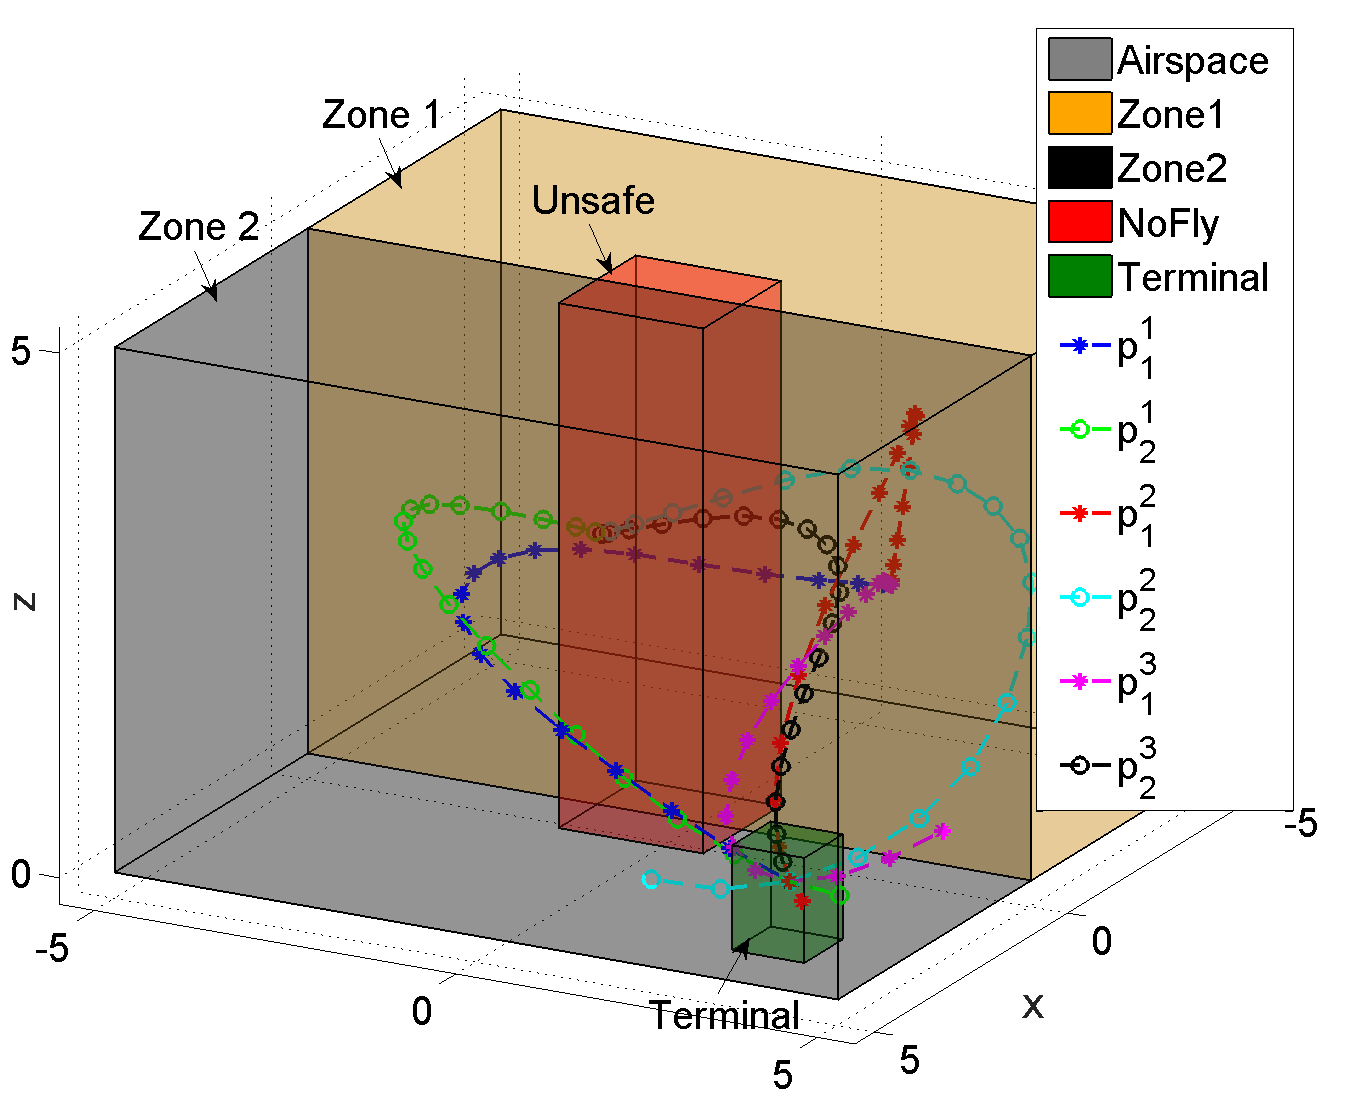
\includegraphics[width=0.49\textwidth]{figures/QuadTrajs_u_scissored}
\vspace{-10pt}
\caption{{\small Trajectories obtained via SQP on smooth robustness, with three different initial trajectories acting as initial solutions for the SQP. Note, all 3 trajectories satisfy $\formula$. Here, $p_{i}^j$ refers to the positions of the $i^{th}$ trajectory for the $j^{th}$ quadrotor. 
%Consider $q_{1}^1$ and $q_{2}^1$, the first trajectory for the two quad-rotors. The second quad-rotor swerves around the obstacle and reaches $\text{Terminal}$, while the first quad-rotor swerves towards $\text{Unsafe}$, without violating $\formula$, in order to maintain a safe distance with the other quad-rotor while reaching $\text{Terminal}$. This results in the two quad-rotors satisfying $\formula$. Similar behavior is seen with the other two trajectories as well. 
A real-time playback of trajectories can be seen in \protect\url{https://youtu.be/FU3Rg1Jb7Fw}.}}
\vspace{-10pt}
\label{fig:quad_ssqp}
\end{figure}


%
\begin{table}[htb]
\small
\begin{center}
\caption{{\small Robustness of final trajectory, $\rob^*$, for 3 runs with different initial trajectories ($\sstraj_0$), none of which satisfy $\formula$.}}
\vspace{-5pt}
\label{tbl:opt_performance}
\begin{tabular} {|c|c|c|c|c|}
	\hline
	\textbf{Run} & $\rob(\sstraj_0) $ &SOP $\rob^* [\srob^*]$ & SA: $\rob^*$ & R-SQP: $\rob^*$\\ \hline
	1 & -0.8803 & \textbf{0.3689}\,[0.4107] & -0.2424 & 0.1798 \\ \hline
	2 & -0.7832 & \textbf{0.3688}\,[0.4106] & -0.5861 & 0.1798 \\ \hline
	3 & -0.0399 & \textbf{0.3689}\,[0.4107] & 0.0854 & 0.1798 \\ \hline
\end{tabular}	
\end{center}
\vspace{-20pt}
\end{table}


